
\documentclass[border=10pt]{standalone}
\usepackage{pgfplots}
\pgfplotsset{compat=1.17}
\usepackage{tikz}
\usetikzlibrary{patterns}
\begin{document}
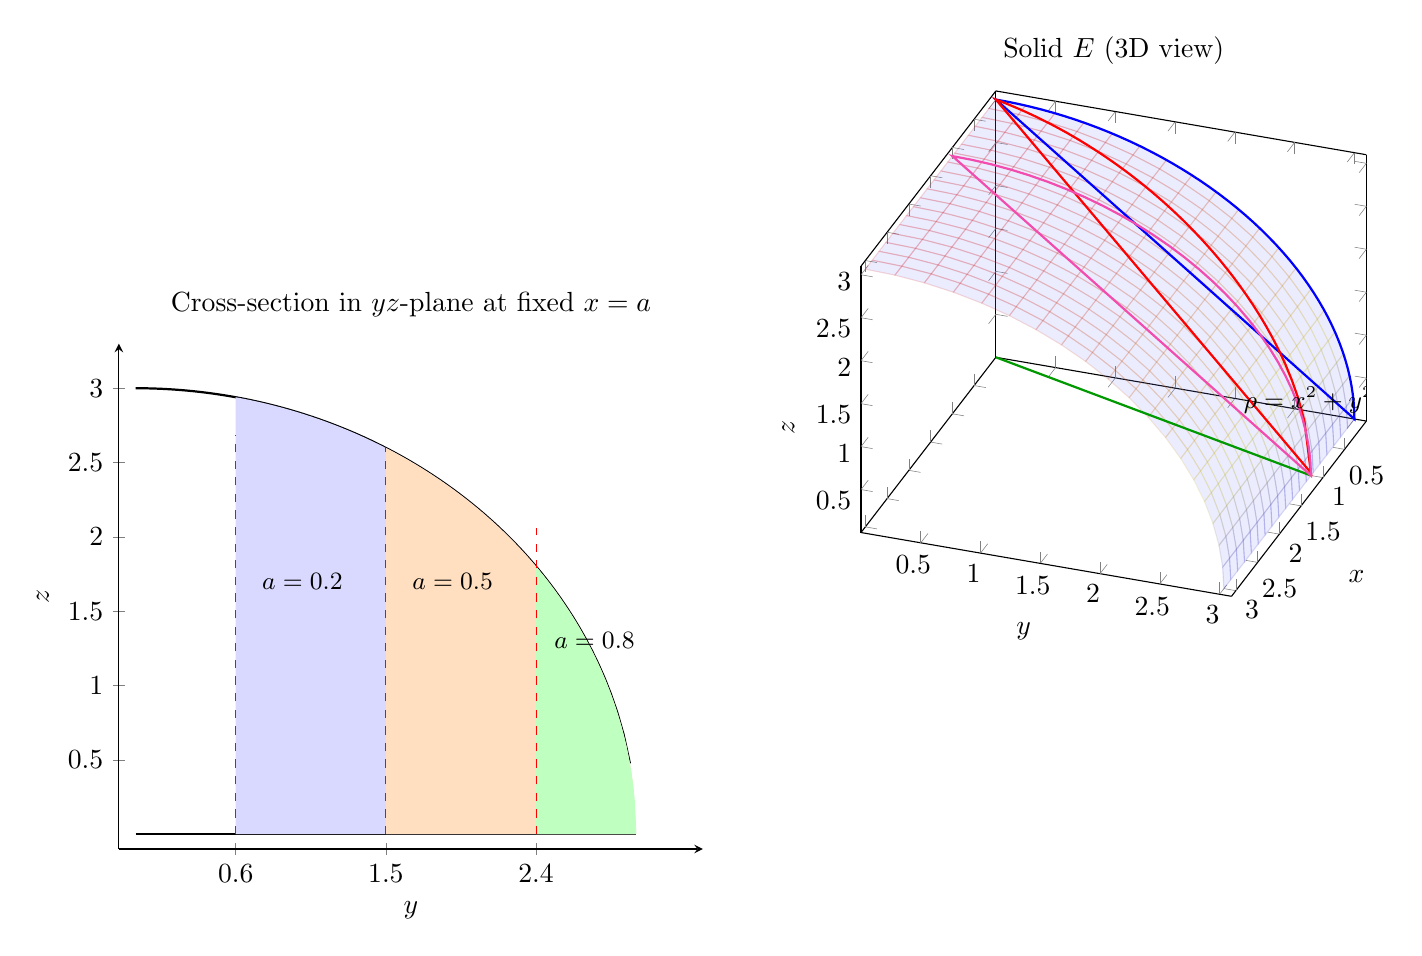
\begin{tikzpicture}

% ----- 2D: yz-cross section showing region E at fixed x = a -----
\begin{axis}[
    name=plot2d,
    xlabel={$y$}, ylabel={$z$},
    xmin=-0.1, xmax=3.4, ymin=-0.1, ymax=3.3,
    width=9cm, height=8cm,
    axis lines=left,
    xtick={0.6, 1.5, 2.4}, ytick={0.5, 1, 1.5, 2, 2.5, 3},
    title={Cross-section in $yz$-plane at fixed $x=a$},
    legend pos=north east,
    samples=80
]
% Quarter disk outline
\addplot[domain=0:3, black, thick] ({x}, {sqrt(9-x^2)});
\addplot[domain=0:3, black, thick] ({x}, 0);

% Region at x = 0.2: y from 0.6 to 3
\addplot[domain=0.6:3, fill=blue!15, draw=none] {sqrt(9-x^2)} \closedcycle;
% Region at x = 0.5: y from 1.5 to 3
\addplot[domain=1.5:3, fill=orange!25, draw=none] {sqrt(9-x^2)} \closedcycle;
% Region at x = 0.8: y from 2.4 to 3
\addplot[domain=2.4:3, fill=green!25, draw=none] {sqrt(9-x^2)} \closedcycle;

% Vertical lines y = 3x for each a
\draw[red, dashed] (axis cs:0.6,0) -- (axis cs:0.6, 2.683);
\draw[red, dashed] (axis cs:1.5,0) -- (axis cs:1.5, 2.598);
\draw[red, dashed] (axis cs:2.4,0) -- (axis cs:2.4, 2.062);

\node at (axis cs:1.0, 1.7) {\small $a=0.2$};
\node at (axis cs:1.9, 1.7) {\small $a=0.5$};
\node at (axis cs:2.75, 1.3) {\small $a=0.8$};

\end{axis}

% ----- 3D schematic on the right -----
\begin{axis}[
    name=plot3d,
    at={(plot2d.right of east)}, xshift=2cm,
    view={110}{35},
    xlabel={$x$}, ylabel={$y$}, zlabel={$z$},
    xmin=0, xmax=3.1, ymin=0, ymax=3.1, zmin=0, zmax=3.1,
    width=8cm, height=8cm,
    title={Solid $E$ (3D view)},
    xtick={0.5,1,1.5,2,2.5,3},
    ytick={0.5,1,1.5,2,2.5,3},
    ztick={0.5,1,1.5,2,2.5,3},
]
% Quarter cylinder surface
\addplot3[
    domain=0:3, domain y=0:1.5708,
    samples=20, samples y=20,
    surf, z buffer=sort, opacity=0.15, color=blue!50
] ({x}, {3*cos(deg(y))}, {3*sin(deg(y))});

% Boundary x = 0: half circle in yz-plane
\addplot3[domain=0:1.5708, samples=50, blue, thick] ({0}, {3*cos(deg(x))}, {3*sin(deg(x))});

% Boundary z = 0: line y from 0 to 3 at z=0
\addplot3[domain=0:3, samples=10, green!60!black, thick] ({x/3}, {x}, {0});

% Edge: intersection of plane y=3x with cylinder (x in [0,1])
\addplot3[domain=0:1, samples=50, red, thick] ({x}, {3*x}, {3*sqrt(1-x^2)});

% Arc at x = 1 (where y=3x meets cylinder)
\addplot3[domain=0:1.5708, samples=30, magenta!70, thick] ({1}, {3*cos(deg(x))}, {3*sin(deg(x))});

\node at (axis cs:0.5, 2.8, 0.5) {\small $\rho = x^2 + y^2$};
\end{axis}

\end{tikzpicture}
\end{document}
